\section{Introduction}

In-context learning adapts a frozen language model (LM) to tasks by conditioning the LM on a textual prompt including task instructions and a few demonstrating examples~\cite{mccann2018natural,radford2019language,brown2020language}. For knowledge-intensive tasks such as question answering, fact checking, and information-seeking dialogue, retrieval models (RM) are increasingly used to augment prompts with relevant information from a large corpus~\citep{lazaridou2022internet,press2022measuring,khot2022decomposed}.


Recent work has shown such \textit{retrieval-augmented in-context learning} to be effective in simple ``retrieve-then-read'' pipelines: a query is fed to the RM and the retrieved passages become part of a prompt that provides context for the LM to use in its response. In this work, we argue that the fact that both LMs and RMs consume (and generate or retrieve) natural language texts creates an opportunity for much more sophisticated interactions between them. Fully realizing this would be transformative: frozen LMs and RMs could serve as infrastructure across tasks, enabling ML- and domain-experts alike to rapidly build grounded AI systems at a high level of abstraction and with lower deployment overheads and annotation costs.

\begin{figure}[!t]
    \centering
    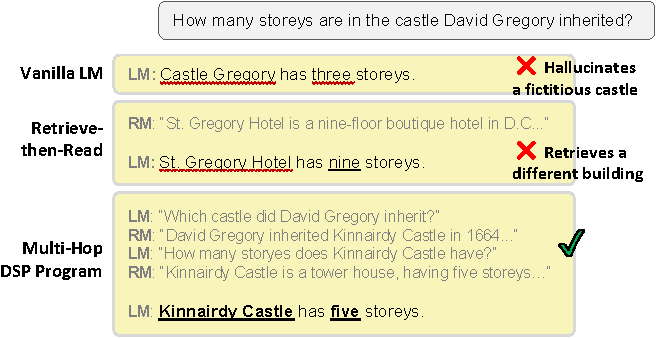
\includegraphics[width=.95\columnwidth]{figures/DSP-tasks.pdf}
    \vspace{-3mm}
    \caption{A comparison between three systems based on GPT-3.5 (\texttt{text-davinci-002}). On its own, the LM often makes false assertions. An increasingly popular retrieve-then-read pipeline fails when simple search can't find an answer. In contrast, a task-aware DSP program successfully decomposes the problem and produces a correct response. Texts edited for presentation.}
    \label{fig:tasks}
    \vspace{-6mm}
\end{figure}


\begin{figure*}[!t]
    \centering
    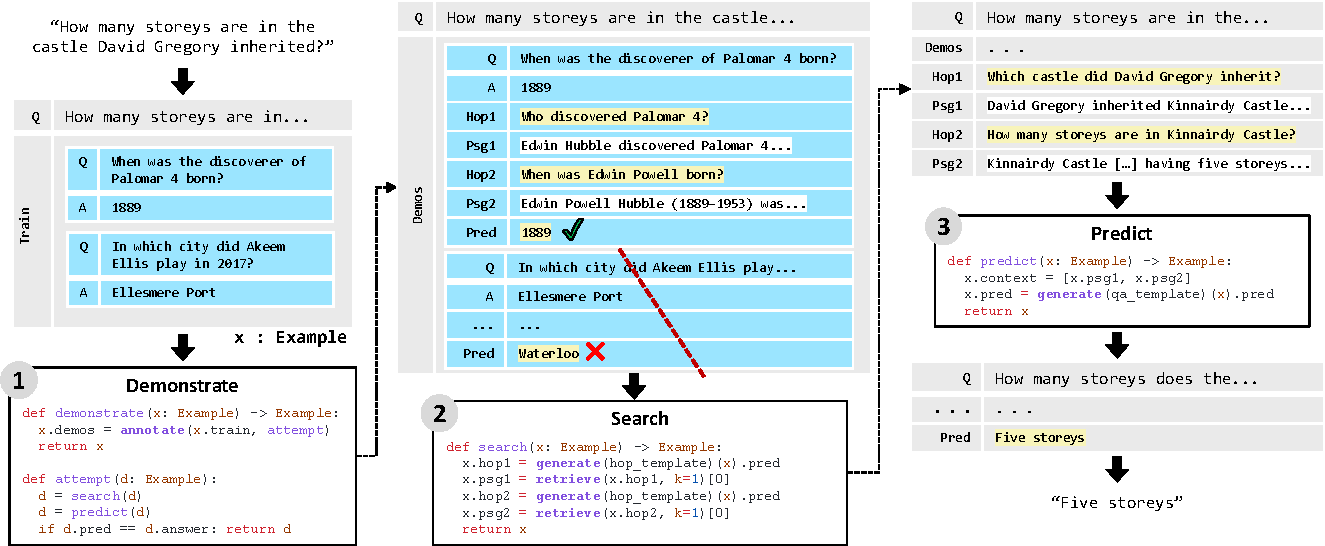
\includegraphics[width=.96\textwidth]{figures/DSP-example.pdf}
    \vspace{-2mm}
    \caption{A toy example of a DSP program for multi-hop question answering. Given an input question and a 2-shot training set, the \demonstrate stage programmatically annotates intermediate transformations on the training examples using a form of weak supervision. Learning from a resulting \textit{demonstration}, the \search stage decomposes the complex input question and retrieves supporting information over two retrieval hops. Finally, the \predict stage uses the demonstration and retrieved passages to answer the question.}
    \label{fig:example}
    \vspace{-3mm}
\end{figure*}

Figure~\ref{fig:tasks} begins to illustrate the power of retrieval-augmented in-context learning, but also the limitations of ``retrieve-then-read'' \cite{lazaridou2022internet,izacard2022few}. Our query is ``How many storeys are in the castle David Gregory inherited?'' When prompted to answer this, GPT-3.5 (\texttt{text-davinci-002}; \citealt{ouyang2022training}) makes up a fictitious castle with incorrect attributes, highlighting the common observation that knowledge stored in LM parameters is often unreliable~\cite{shuster2021retrieval,ishii2022survey}.
Introducing an \RM{} component helps, as the \LM{} can ground its responses in retrieved passages, but a rigid retrieve-then-read strategy fails because the \RM{} cannot find passages that directly answer the question.

We introduce the \textbf{\demonstrate--\search--\predict} (\textbf{\DSP}) framework for in-context learning, which relies entirely on passing natural language text (and scores) between a frozen \RM{} and \LM{}. \DSP introduces a number of composable functions that bootstrap training examples (\demonstrate), gather information from a knowledge corpus (\search), and generate grounded outputs (\predict), using them to systematically unify techniques from the retrieval-augmented NLP and the in-context learning literatures~\citep{lee2019latent,khattab2021baleen,anantha2020open,gao2022attributed,izacard2022few,dohan2022language,zelikman2022star,zhang2022automatic}. 
We use \DSP to suggest powerful %
strategies for knowledge-intensive tasks with compositions of these techniques. This reveals new conceptual possibilities for in-context learning in general (\secref{sec:dsp}), and it allows us to present rich programs that set new state-of-the-art results (\secref{sec:eval}).






Figure~\ref{fig:tasks} shows the path that a \DSP program might take to arrive at an answer, and Figure~\ref{fig:example} illustrates how a deliberate program achieves this. Instead of asking the \LM{} to answer this complex question, the program's \search stage uses the \LM{} to generate a query ``Which castle did David Gregory inherit?'' The \RM{} retrieves a passage saying Gregory inherited the Kinnairdy Castle. After a second search ``hop'' finds the castle's number of storeys, the \predict stage queries the \LM{} with these passages to answer the original question. Although this program implements behaviors such as query generation, it requires no hand-labeled examples of these intermediate \textit{transformations} (i.e., of the queries and passages of both retrieval hops). Instead, the \demonstrate stage uses labeled question--answer pairs to implement a form of weak supervision that programmatically annotates the transformations invoked within \search and \predict.



We evaluate several \DSP programs on answering questions in open-domain, multi-hop, and conversational settings. In them, we implement novel and reusable transformations such as bootstrapping annotations for all of our pipelines with weak supervision (\secref{sec:dsp:demonstrate}), reliably rewriting questions to resolve conversational dependencies and iteratively decompose complex queries with summarization of intermediate hops (\secref{sec:dsp:search}), and generating grounded responses from multiple passages with self-consistency (\secref{sec:dsp:predict}). We report preliminary results on Open-SQuAD, HotPotQA, and QReCC using the frozen \LM{} GPT-3.5 and \RM{} ColBERTv2~\cite{khattab2020colbert,santhanam-etal-2022-colbertv2} with no fine-tuning. Our \DSP programs deliver 37--120\%, 8--39\%, and 80--290\% relative gains against corresponding vanilla LMs, a standard retrieve-then-read pipeline, and a contemporaneous self-ask pipeline \citep{press2022measuring}, respectively.
Future versions of this report will include additional test tasks and \LM\ choices.



In summary, this work makes the following contributions. First, we argue that simple task-agnostic pipelines for in-context learning should give way to deliberate, task-aware strategies. Second, we show that this shift need not be a burden: with \DSP, such strategies can be easily expressed as short programs using composable operators. Third, this composability spawns powerful capacities, like automatically annotating demonstrations for complex pipelines from end-task labels. Fourth, for three knowledge-intensive tasks, we implement rich programs that establish state-of-the-art results for in-context learning.




























  









